\section{Introduction}
\label{sec:introduction}

% state the learning objective 


The objective of this laboratory assignment is to study a circuit containing dependent and independent Voltage and Current Sources connected to resistors, and to improve our skills on managing all the three sotwares used in this assignement.

The circuit in question is depicted in Figure~\ref{fig:circuit}
\begin{figure}
  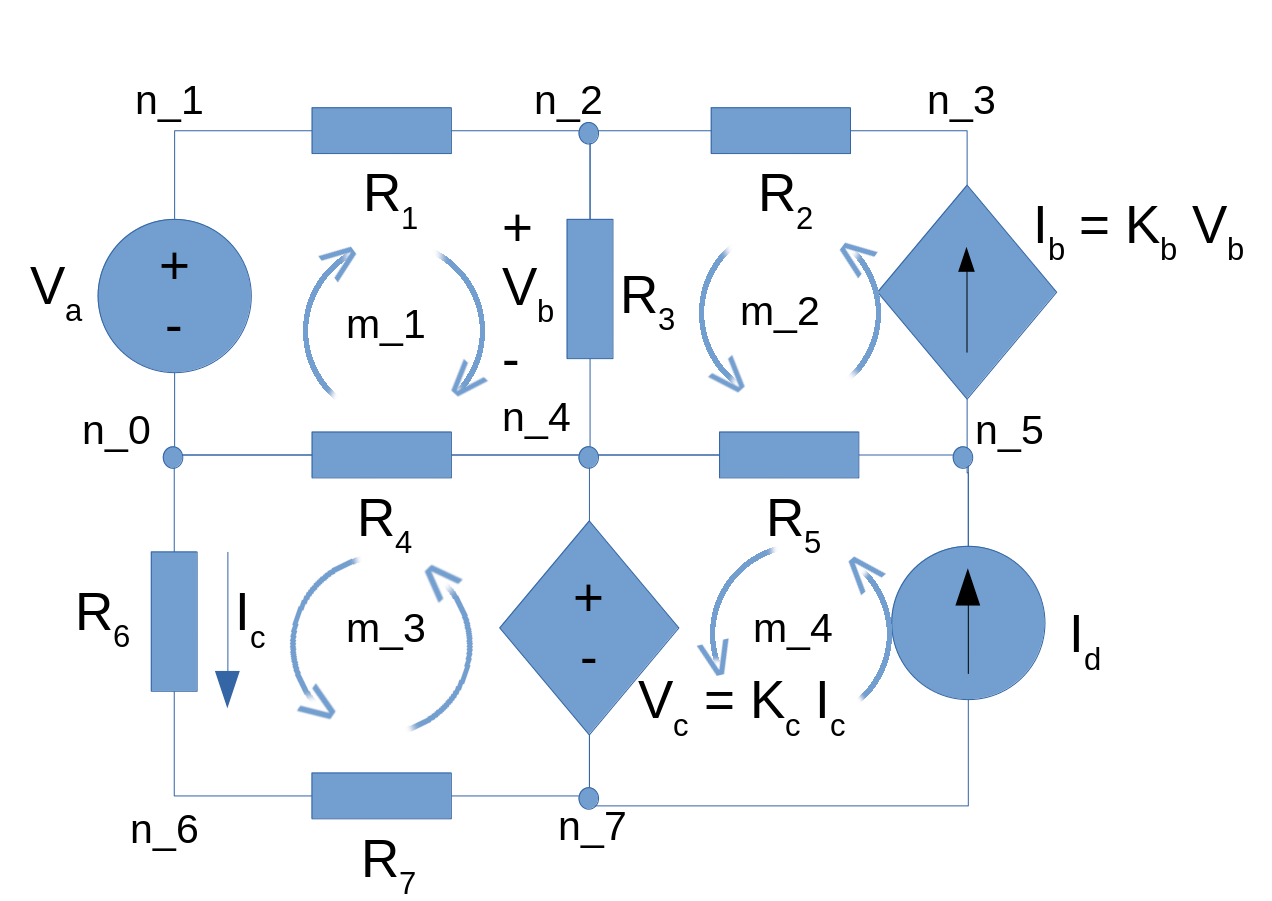
\includegraphics[width=\linewidth]{circuit.png}
  \caption{The circuit with the mesh currents represented by circular arrows}
  \label{fig:circuit}
\end{figure}
%%%%%%%%%%%%%%%%%%%descobrir o q esta mal aqui

In Section~\ref{sec:analysis}, a theoretical analysis of the circuit, using GNU Octave,  is presented. In Section~\ref{sec:simulation}, the circuit is simulated, and the results are compared to the theoretical ones from
aforementioned one. The conclusions of the study are presented in the last section of the document.
